\section{\PwTerTITLE: automatic litmus test evaluator}
\label{sec:tool}

\PwTer{} automatically and exhaustively calculates the allowed outcomes of litmus tests for the \PwT, \PwTpo, and \PwTc{} models. It is built in OCaml, and uses Z3~\cite{Z3Solver} to judge the truth of predicates constructed by the models. \PwTer{} obviates the need for error-prone hand evaluation.

\PwTer{} allows several modes of evaluation: it can evaluate the rules of Fig.~\ref{fig:seq}, implementing \PwT; it can generate program order according to \textsection\ref{sec:c11}, implementing \PwTpo; and similar to \MRD~\cite{DBLP:conf/esop/PaviottiCPWOB20}, it can construct C11-style pre-executions and filter them according to the rules of \rcXI{} as described in \textsection\ref{sec:c11}.
Finally, \PwTer{} also allows us to toggle the complete check of~\ref{def:complete}, providing an interface for understanding how fragments of code might compose by exposing preconditions and termination conditions that are not yet tautologies.
% We show \PwTer{} in action in Fig.~\ref{fig:tool}. 
\PwTer{} will be made open source upon publication.
%\PwTer{} is available online at \url{https://github.com/graymalkin/pomsets-with-predicate-transformers}.

%% [Simon] I am not a fan of how this looks on the page.
% \begin{figure}[t]
% \begin{center}
%   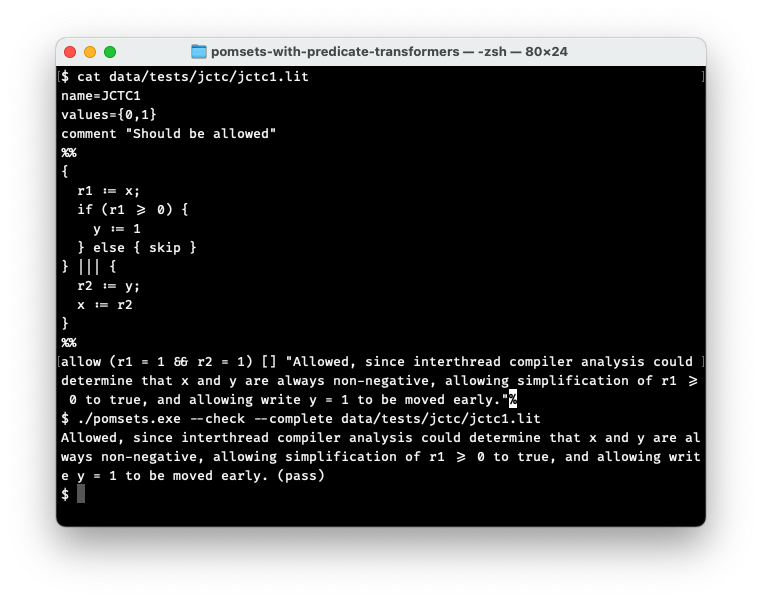
\includegraphics[width=0.75\textwidth]{tool.png}
%   \Description{Image shows tool running on a Mac. Java Causality Test Case 1 is printed, followed by an invocation of the tool as {\tt ./pomsets.exe --check --complete data/tests/jctc/jctc1.lit}, which shows that the tool passes the assertion listed in the test.}
%   \caption{\label{fig:tool} Example output of \PwTer, validating TC1~\cite{PughWebsite}.}
% \end{center}
% \end{figure}
